\begin{frame}
  \frametitle{Метод шагающих кубиков}

  \begin{block}{Триангуляция}
    Для получения полигонизированной поверхности необходимо:
    \begin{enumerate}
      \item Создать сетку вокселей, каждый узел которой обладает потенциалом меньше или больше заданного;
      \item Получить базовые треугольники для данного случая;
      \item Уточнить вершины треугольников интерполяцией.
    \end{enumerate}
  \end{block}

  \begin{block}{Базовые треугольники}
    \begin{center}
      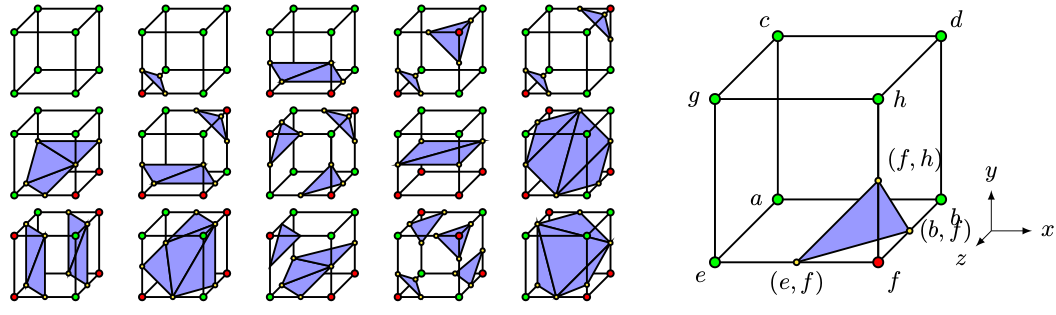
\includegraphics[height=.3\paperheight]{marching-cubes.png}
    \end{center}
  \end{block}
\end{frame}

\begin{frame}
  \frametitle{Потенциалы}

  \begin{block}{Проблема}
    Для применения метода шагающих кубиков необходимо иметь потенциалы в узлах сетки, однако мы имеем разрозненные частицы, несвязанные никакой структурой.
  \end{block}

  \begin{block}{Решение}
    \begin{enumerate}
      \item Для каждой частицы определить занимаемый воксель;
      \item Увеличить счётчик частиц в данном вокселе;
      \item Вычислить потенциалы в узлах усреднением прилежащих восьми вокселей.
    \end{enumerate}
  \end{block}
\end{frame}

\begin{frame}
  \frametitle{Гистограммные пирамиды}

  \begin{block}{}
    Триангулировать имеет смысл только непустые воксели, которых немного. Для их поиска используются гистопирамиды.
  \end{block}

  \begin{columns}[onlytextwidth]
    \begin{column}{.55\textwidth}
      \begin{block}{Создание пирамиды}
        \begin{center}
          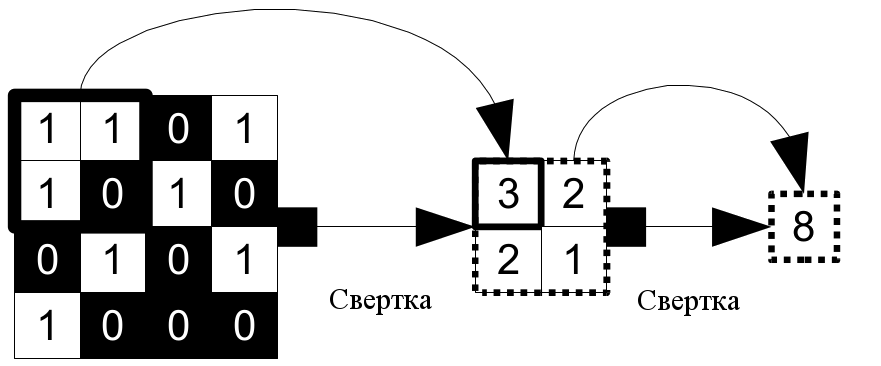
\includegraphics[width=\textwidth]{histopyramid-builder.png}
        \end{center}
        На последнем уровне имеем количество непустых вокселей.
      \end{block}
    \end{column}
    \begin{column}{.35\textwidth}
      \begin{block}{Заполнение списка \\ непустых вокселей}
        \centering
        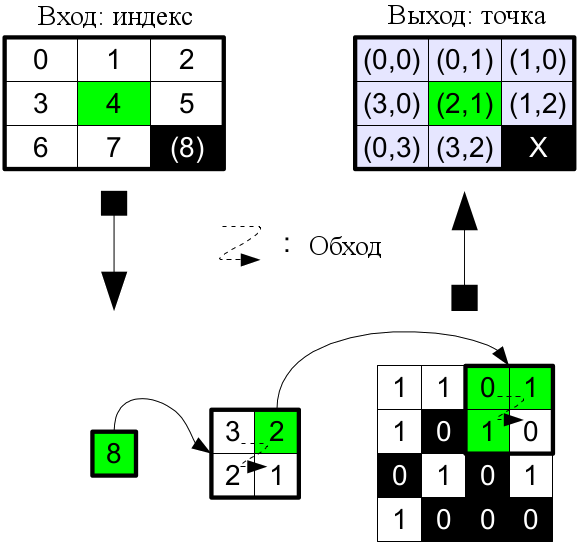
\includegraphics[width=\textwidth]{pointlist-builder.png}
      \end{block}
    \end{column}
  \end{columns}
\end{frame}
